\subsection{Сила, работа и потенциальная энергия. Консервативные и неконсервативные силы. Работа и кинетическая энергия. Закон сохранения полной механической энергии в поле потенциальных сил}

\begin{definition}
    Сила $[F, Н]$ — векторная величина, являющаяся мерой воздействия на данное тело со стороны других тел или полей
\end{definition}

$$\vec F=\frac{d(m\vec\upsilon)}{dt}$$ 
$$F=ma$$

\begin{definition}
    Работа $[A, Дж]$ — скалярная количественная мера действия силы (равнодействующей сил) на тело.
\end{definition}

$$A=FScos\alpha$$

$$A_{12}=\int\limits_{\vec{r_1}}^{\vec{r_2}}\vec F\ d\vec r$$

\begin{definition}
    Потенциальная энергия $[E_П, Дж]$ — скалярная величина, представляющая собой часть полной механической энергии системы, находящейся в поле консервативных сил.
\end{definition}

$$E_П=mgh$$

\begin{definition}
    Консервативные силы — силы, работа которых при перемещении тела от точки $1$ к точке $2$ 
    зависит не от траектории движения этого тела между точками, а только от положения этих точек.
\end{definition}

Для консервативных сил можно ввести потенциальную энергию $E_П$. В механике до этого уже имеется кинетическая энергия $E_K$.

Консервативные силы:

\begin{itemize}
    \item Сила тяжести
    $$A=-\int_{h1}^{h2}mg\ dh=mg(h_1-h_2)$$
    \item Сила упругости
    $$A=-\int_0^xkx\ dx=-\frac{kx^2}{2}$$
    \item Сила гравитации
    $$F=G\frac{m_1m_2}{r^2}$$
    \item Сила электростатического взаимодействия
    $$F=k\frac{q_1q_2}{r^2}$$
\end{itemize}

\begin{definition}
    Неконсервативные (диссипативные) силы — все остальные силы, чья работа вычисляется по пути.

    Проще говоря, неконсервативные - те, что “тратят” энергию системы на какие-то другие процессы.
\end{definition}

Неконсервативные силы:
\begin{itemize}
    \item Сила трения
        $$F=\mu N$$
    \item Сила сопротивления воздуха
        $$F=k\upsilon^2$$
\end{itemize}

\begin{definition}
    Механическая энергия характеризует способность тела совершать работу.

    Кинетическая энергия $[E_K, Дж]$ — энергия движения, которая зависит от массы тела, величины скорости и не зависит от положения тела в пространстве.
\end{definition}

$$E_K=\frac{m\upsilon^2}{2}$$

\begin{definition}
    Работа — это физическая величина, являющаяся скалярной количественной мерой действия 
    силы или сил на тело или систему, зависящая от численной величины, направления силы (сил) и от перемещения точки (точек) тела или системы. 
\end{definition}

\begin{definition}
    Работа неконсервативной силы — изменение кинетической энергии тела:

    $$A=E_{K_2}-E_{K_1}=\Delta E_K$$
\end{definition}

Если $A>0$, то $\Delta E_K>0$ - кинетическая энергия возрастает
Если $A<0$, то $\Delta E_K<0$ - кинетическая энергия убывает

\begin{definition}
    Потенциальная энергия — энергия взаимодействия, которая зависит от положения тел или частей тела друг относительно друга.

    Если в системе действует консервативные силы, то система обладает потенциальной энергией. Поэтому консервативные силы называют потенциальными.

    Если консервативные силы совершают работу, то положение тел в системе меняется и потенциальная энергия системы тоже изменяется.
\end{definition}

\begin{definition}
    Работа консервативных сил — убыль потенциальной энергии:

    $$
    A=E_{п1}-E_{п2}=-\Delta E_{п}
    $$
\end{definition}

\begin{definition}
    Полная механическая энергия:

    $$
    E=E_П+E_K
    $$
\end{definition}

\begin{definition}
    Закон сохранения энергии  — в любых явлениях природы энергия не исчезает и не возникает, а только переходит из одного вида в другой в эквивалентных количествах.

    Закон сохранения энергии  — в замкнутой системе тел, между которыми действуют только консервативные силы, полная механическая энергия остаётся постоянной при любых процессах внутри системы.

    Рассмотрим замкнутую систему тел, между которыми действуют только консервативные силы. Соответственно, каждое состояние характеризуется кинетической и потенциальной энергией.

    При переходе системы из одного состояния в другое силы, приложенные к телам, совершают работу.
\end{definition}

Работа консервативных сил с одной стороны равна увеличению кинетической энергии, а с другой - убыли потенциальной энергии, т.е.:

\begin{figure}[h]
    \centering
    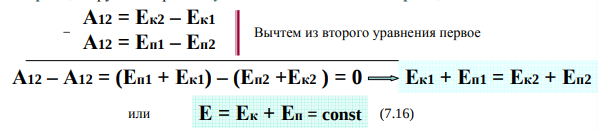
\includegraphics[width=0.7\linewidth]{imgs/q7i1.png}
\end{figure}